% !TeX encoding=utf8
% !TeX spellcheck = de_CH_frami

\chapter{Recherche}
In diesem Kapitel werden die Grundlagen recherchiert wie die beiden Teilprojekte "`Sensordaten sammeln"' und "`Sensordaten auswerten (BigData)"' angegangen werden könnten.

\section{Ausgangslage}
Die Vorlesung zu diesem Semniar befasst sich mit den Konzepten der Funktionalen Programmierung. Zur Veranschaulichung dieser Konzepte wurde die Programmiersprache F\# des .NET-Frameworks verwendet. Aufgrund dessen haben wir uns entschieden auch dieses Seminar mit der uns bekannten funktionalen Programmiersprache F\# umzusetzen. Als \Gls{gls:iot} Gerät wird ein Raspberry Pi\footcite{Raspberry_Pi_2016-04-24} verwendet. Der Raspberry Pi ist ein Einplatinencomputer welcher von der britischen Raspberry Pi Foundation entwickelt wurde. Der Raspberry Pi bietet den Vorteil, dass er sehr weit verbreitet ist\footcite{Raspberry_Pi_Erfolgsgeschichte_2016-04-24}, er kostengünstig ist und es inzwischen eine sehr grosse Anzahl an verschiedenen Sensoren auf dem Markt gibt mit welchen Daten gesammelt werden können\footcite{Raspberry_Pi_Sensor_2016-04-24}.

\section{Der Raspberry Pi}
\label{sec:recherche:rpi}
\begin{figure}[H]
  \centering
  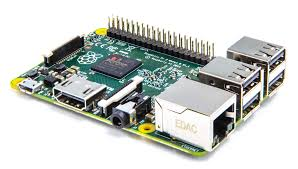
\includegraphics[width=9cm]{./images/RaspberryPi2ModelB}
  \captionsource{Raspberry Pi 2 Model B}{\url{https://www.raspberrypi.org/wp-content/uploads/2015/01/Pi2ModB1GB_-comp.jpeg}}
\end{figure}
  
Wie bereits im vorangehenden Kapitel beschrieben, handelt es sich beim Raspberry Pi um einen Einplatinencomputer welcher von der Raspberry Pi Foundation entwickelt und vertrieben wird. Er hat ungefähr die Grösse einer Kreditkarte und bietet zahlreiche On-Board Schnittstellen wie USB-, HDMI und Audio Anschlüsse (Abhängig vom konkreten Modell). Zusätzlich stehen eine bestimmte Anzahl an GPIO-Pins (General Purpose Input / Output) zur Verfügung. Mit Hilfe dieser Pins lassen sich zum einen Erweiterungs-Boards anschliessen und zum anderen können auch eigene Schaltungen, etc. gebaut und verlötet werden. Die Anzahl und genaue Funktion der einzelnen GPIO-Pins ist vom konkreten Raspberry Pi Modell abhängig.

Am 29 Februar 2016 ist die neuste Version, der Raspberry Pi 3 (Model B), auf dem Markt erschienen\footcite{Raspberry_Pi_3_2016-04-24}. Einige Zahlen zu dem Gerät:

\begin{itemize}
\item 1.2GHz 64-bit quad-core ARM Cortex-A53 CPU (Leistungsteigerung: ~10x des Raspberry Pi 1 und ~1.6x des Raspberry Pi 2)
\item Integriertes 802.11n wireless LAN und Bluetooth 4.1
\item Vollständige Kompatibilität zu Version 1 und 2 des Raspberry Pi (Model B)
\end{itemize} 


\begin{figure}[H]
  \centering
  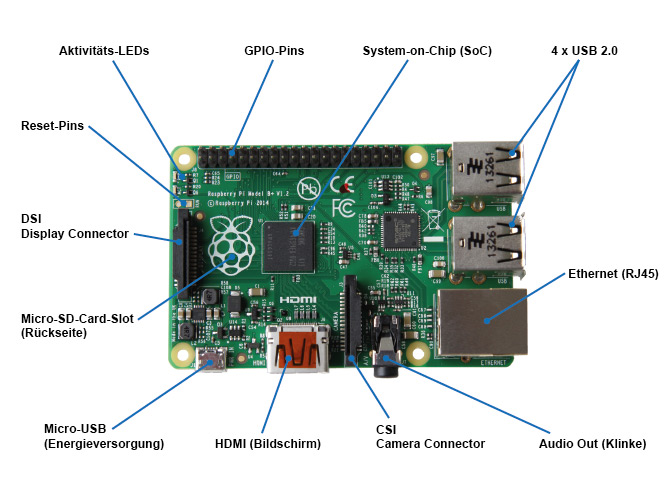
\includegraphics[width=13cm]{./images/RaspberryPi2ModelBPlusOverview}
  \captionsource{Raspberry Pi 2 Model B Überblick}{\url{https://www.elektronik-kompendium.de/sites/raspberry-pi/bilder/19052512.jpg}}
\end{figure}

\newpage
\begin{landscape}

\subsection{Raspberry Pi Modelle im Überblick}
\begin{table}[H]
\centering
\begin{tabular}{r | c  | c | c | c | c | c | c | c | c | c}
	& \THrot{\textbf{Raspberry Pi Model A}}
	& \THrot{\textbf{Raspberry Pi Model A+}}
	& \THrot{\textbf{Raspberry Pi Model B}}
	& \THrot{\textbf{Raspberry Pi Model B+}}
	& \THrot{\textbf{Raspberry Pi 2 Model B}}
	& \THrot{\textbf{Raspberry Pi 3 Model B}}
	& \THrot{\textbf{Raspberry Pi Compute}}
	& \THrot{\textbf{Raspberry Pi Zero}}\\
\midrule
Gewicht in Gramm
	& 	31
	&	23
	&	40		
	& 	45 
	&	40
	&	40
	&	7
	&	9\\
\midrule
System-on-a-Chip (SoC):
	& 	\multicolumn{4}{|c|}{BCM2835} 
	&	BCM2836
	&	BCM2837
	&	\multicolumn{2}{|c|}{BCM2835} \\
\midrule
CPU Kerne
	& 	1
	&	1
	&	1		
	& 	1 
	&	1
	&	4
	&	1
	&	1\\
\midrule
CPU Takt in MHz
	& 	\multicolumn{4}{|c|}{700} 
	&	900
	&	1200
	&	700
	&	1000\\
\midrule
CPU Architektur
	& 	\multicolumn{4}{|c|}{ARMv6 (32-bit)}  
	&	ARMv7 (32-bit)	
	&	ARMv7 (64-bit)	
	&	\multicolumn{2}{|c|}{ARMv6 (32-bit)}  	\\
\midrule
GPU Takt in MHz
	& 	\multicolumn{5}{|c|}{250} 
	&	300/400
	&	\multicolumn{2}{|c|}{250} \\
\midrule
Arbeitsspeicher in MB
	& 	\multicolumn{2}{|c|}{256}  
	&	256 / 512		
	& 	\multicolumn{2}{|c|}{512}  	
	& 	1024 
	&	\multicolumn{2}{|c|}{512}  	\\
	
\midrule
Pins
	& 	26
	&	40
	& 	26
	& 	\multicolumn{3}{|c|}{40}  	
	&	60
	&	40  	\\
	
\midrule
GPIO-Pins
	& 	17	
	&	26
	& 	17
	& 	\multicolumn{3}{|c|}{26}  	
	&	48
	&	26  	\\
\bottomrule
\end{tabular}
\end{table}

\end{landscape}
\newpage

\section{F\# mit dem Raspberry Pi}
\label{sec:recherche:fsharprpi}
Um F\# auf dem dem Raspberry Pi auszuführen, gibt es grundsätzlich zwei Möglichkeiten, welche nachfolgend erläutert werden.
Da es sich bei F\# um eine Sprache des Microsoft .NET-Frameworks handelt, wird für die Ausführung zwingend eine Implementation des .NET-Frameworks benötigt.

\subsection{Linux (Raspbian)}
Ein weit verbreitetes Betriebsystem für den Raspberry Pi ist das Raspbian\footcite{FrontPage_-_Raspbian_2016-04-24} OS. Bei dem Namen handelt es sich um eine Kombination von Raspberry und Debian. Demnach handelt es sich auch um eine Debian Distribution, welche spezifisch für den Raspberry Pi entwickelt wurde.

Eine Möglichkeit um unter Linux, beziehungsweise Raspbian, F\# auszuführen ist das Mono-Framework\footcite{Mono_2016-04-24}. Dabei handelt es sich um eine Open Source Implementation von Microsoft's .NET Framework.

\subsection{Windows 10 IoT}
Microsoft hat mit Windows 10 IoT eine Version ihres Betriebssystem herausgebracht, welche speziell für leistungsschwächere Geräte entwickelt wurde\footcite{Windows_IoT_2016-04-24}. Bei der IoT Version von Windows 10 ist das .NET Framework bereits standardmässig an Bord. Demnach sollte es keine Probleme geben um F\# auf dieser Plattform zu betreiben.

\section{GrovePi Sensoren}
Für den Raspberry Pi gibt es viele verschiedene Sensoren auf dem Markt. Herauskristallisiert hat sich jedoch das Starter Kid GrovePi+\footcite{GrovePi_2016-04-24}. Dieses beinhaltet unter anderem Ton-, Temperatur-, Feuchtigkeit- und Lichtsensoren. Der Vorteil an den GrovePi Sensoren besteht an den geringen Kosten, dem einfachen Anschluss an den Raspberry Pi und die vielen verfügbaren Beispiele in unterschiedlichsten Programmiersprachen (z.B. Java, Python, C, C++).

Die Recherchen haben ebenfalls gezeigt, dass es eine Library für .NET gibt mit welchem die Sensoren angesprochen werden können\footcite{NuGet_GrovePi_2016-04-24}.

\section{Verwendete Hardware für die Umsetzung}
Wir haben uns entschieden für die Umsetzung die nachfolgend aufgelisteten Hardware-Komponenten zu verwenden:
\begin{itemize}
\item Raspberry Pi 2 Model B
\item Raspberry Pi 3 Model B
\item GrovePi Sensoren
\begin{itemize}
\item Temperature \& Humidity Sensor
\item Sound Sensor
\item Light Sensor
\item Blue LED
\end{itemize}
\end{itemize}

\section{Datenauswertung}
Die von den Sensoren gespeicherten Daten werden in einem noch zu definierenden Format abgespeichert und danach für die Datenauswertung ausgelesen. Dafür wurde vom Dozenten die Library F\# Data empfohlen\footcite{Fsharp_Data_2016-04-24}. Diese kann Daten in den Formaten \gls{acr:CSV}, \gls{acr:HTML}, \gls{acr:JSON} und \gls{acr:XML} entgegennehmen und verarbeiten.

